\section{Task 3}
\begin{align*}
    v_1 &= \cos(x) \\ 
    v_2 &= x^5 \\ 
    v_3 &= v_1-v_2 \\ 
    v_4 &= x^3 \\ 
    y &= \frac{v_3}{v_4}
\end{align*}
Therefore:
\begin{align*}
    \tilde{v_1} &= \cos(x) (1+\eta_1)\\ 
    \tilde{v_2} &= x^5(1+\eta_2)\\ 
    \tilde{v_3} &= (\tilde{v_3} - \tilde{v_4})(1+\eta_3) \\ 
    \tilde{v_4} &= x^3 (1+\eta_4) \\
    \tilde{y} &= \frac{\tilde{v_3}}{\tilde{v_4}}(1+\eta_5)
\end{align*}
\subsection{Epsilon calculus}
Using the epsilon calculus rules:
\begin{align*}
    \tilde{y} &= \left(
    \displaystyle\frac{\cos(x)(1+\eta_1) - x^5(1+\eta_2)(1+\eta_3)}
    {x^3(1+\eta_4)}
    \right) (1+\eta_5) \\
    &=\displaystyle\frac{\cos(x)(1+\eta_1+\eta_3-\eta_4+\eta_5)-
    x^5(1+\eta_2+\eta_3-\eta_4+\eta_5)}{x^3}\\
    &=\displaystyle\frac{\cos(x)+cos(x)(\eta_1+\eta_3-\eta_4+\eta_5)-
    x^5-x^5(\eta_2+\eta_3-\eta_4+\eta_5)}{x^3}\\
    &=y+\displaystyle\frac{cos(x)\eta_1+cos(x)(\eta_3-\eta_4+\eta_5)-
    x^5\eta_2-x^5(\eta_3-\eta_4+\eta_5)}{x^3}\\
    &=y+\displaystyle\frac{cos(x)\eta_1-x^5\eta_2+
    (cos(x)-x^5)(\eta_3-\eta_4+\eta_5)}{x^3}\\
    &=y\cdot\left(1+\frac{cos(x)}{x^3}\frac1y\eta_1-x^2\frac1y\eta_2+
    \frac{cos(x)-x^5}{x^3}\frac1y(\eta_3-\eta_4+\eta_5)\right)\\
\end{align*}
Finally, we get:
$$ K_{A2} = \displaystyle\frac{
    \left|\frac{\cos(x)}{x^3}\right| + \left|-x^2\right|
+ \left| \frac{\cos(x)-x^5}{x^3} \right|
+ \left|-\frac{\cos(x)-x^5}{x^3} \right|
+ \left| \frac{\cos(x)-x^5}{x^3} \right|
} {\left|\frac{\cos(x)}{x^3} - x^2\right|}
$$

\subsection{Numerical simulation}
This part is identical to the corresponding one in Task 2. Of course the
components of the equation change but overall there is nothing to explain
further.

\subsection{Comparison of results}
Similarly to results of task 2, both methods do not differ significantly from
one another in terms of results. This can be seen on \ref{fig:task3}, where the
output difference cannot even be seen (due to one point drawn on the other).

\begin{figure}[ht]
    \begin{center}
        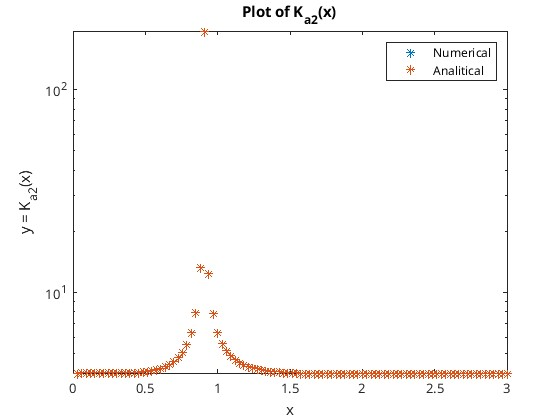
\includegraphics[width=\textwidth]{Task3.jpg}
    \end{center}
    \caption{Comparison of calculating error via numerical and analytical way}
    \label{fig:task3}
\end{figure}
